\documentclass{article}
\usepackage[utf8]{inputenc}

\title{Survey on Discrete Wavelet Transforms Using GPU}
\author{Samuel Li}
\date{April 2015}

%\usepackage{natbib}
\usepackage{graphicx}
\usepackage{color}
\usepackage{setspace}
\newcommand{\fix}[1]{\textcolor{red}{#1}} %Put words in Red

\begin{document}
\onehalfspacing

\maketitle

\begin{abstract}
Discrete Wavelet Transform (DWT) is widely used in data reduction applications.
%
However, such transforms are relatively computationally intensive.
%
To accelerate the calculation of DWT, researchers have applied various parallel
computing techniques, based on the distributed memory architecture~\cite{
chadha2002scalable, woo1995parallel, uhl1996wavelet, nielsen1997scalable}
and the shared memory architecture~\cite{
kutil1999hardware,lucka2000parallel}.
%
In the recent years, the many-core architecture, such as GPU acceleration 
cards, have emerged in the parallel computing field.
%
In this survey paper, we cover many topics regarding calculation of DWT on GPUs.
%
More specifically, we start the survey from technical discussion and evaluation
of implementing the DWT on GPUs~\cite{tenllado2008parallel, van2011accelerating,
garcia2005gpu}.
%
Then we present a few successful use cases of GPU in parallel DWT~\cite{
strengert2004hierarchical, strengert2006pyramid, wong2007discrete,
treib2012turbulence}.
%
Finally, to prepare for the exascale computing, we survey the use of 
heterogeneous architecture with GPUs and multi-core CPUs together,
as well as the GPU clusters~\cite{franco2009parallel, franco2010parallel,
strengert2005large, franco20122d, rossinelli2011multicore}.
%
\end{abstract}

\section{Introduction}

\section{Background of Wavelet Transforms}
Discrete Wavelet Transform (DWT) on a signal $x[n] \: (0 \leq n < N)$ is essentially
passing the signal through a filter function, $f$, 
in a convolution operator.
%
This filter function is also called the \textit{kernel} of this DWT.
%
The results of this DWT are \textit{coefficients} of the signal.
%
The coefficients can be further categorized as two separate groups: 
one representing an approximation of the original signal,
namely \textit{scale coefficients};
and another one contains the detailed information to reconstruct
the original signal from the approximation, namely 
\textit{detail coefficients}.
%
Normally each of these two groups of coefficients has a size $\frac{N}{2}$.


DWTs can also be applied on the coefficients from previous DWTs.
%
When applying another round of DWT, transforms are applied on the two
groups of coefficients separately.
%
As a result, the original singal $x[n]$ is represented as 4 groups of 
coefficients; each has a size $\frac{N}{4}$.
%
This iteration finishes when each of the coefficient groups are small enough,
or the number of iterations reaches the maxinum value set by the user. 
%
%Since a singal is decomposed into multiple groups of coefficients,
%this process is also named a \textit{decomposition}.
%
%Similarly, the reverse calculation, which reconstructs the original signal 
%from the coefficients, is named \textit{reconstruction}.
%
Figure~\ref{fig:example1} illustrates an example of applying DWTs for 
three rounds on an 8-element signal.



\begin{figure}[p]
    \centering
    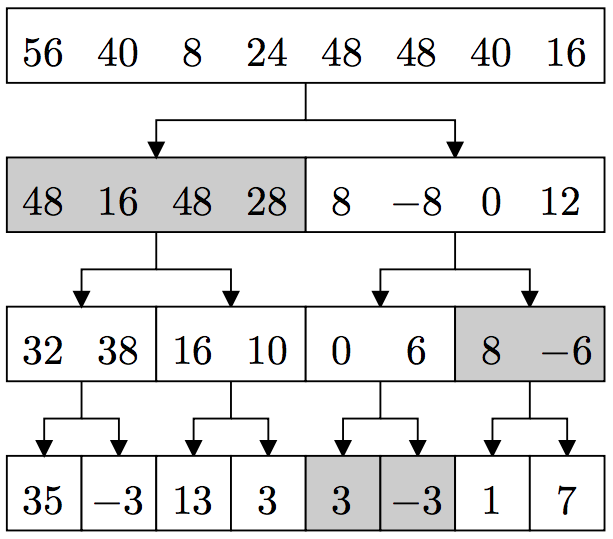
\includegraphics[width=0.8\textwidth]{fig/example1.png}
    \caption{An example of DWT on a signal with 8 elements.}
    \label{fig:example1}
\end{figure}



From the perspective of computational models in parallel computing, 
stencil



\label{sec:bg}

\section{Single Instruction Multiple Data}
The Single Instruction Multiple Data (SIMD) architecture was popular in the
1990s.
%
With SIMD architecture, all processing elements (PE) execute identical instructions
cycle by cycle, but they access different local data from their private 
local memory.
%
All PEs are also connected in a net structure, allowing
communication between them.
%
Figure~\ref{fig:simd1} illustrates an example SIMD architecture.

\begin{figure}
    \centering
    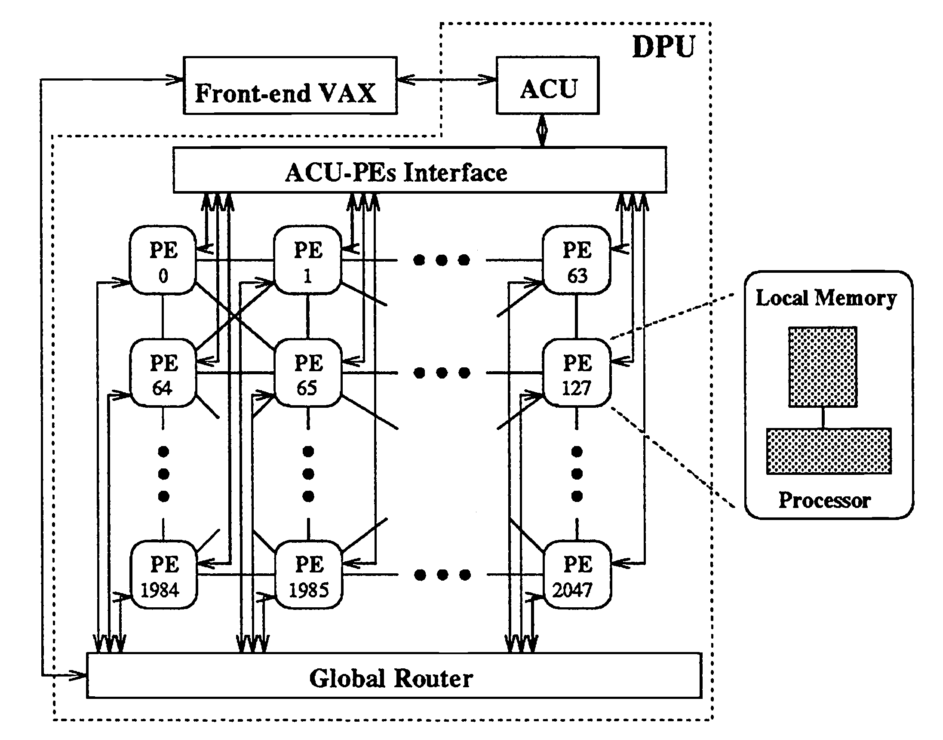
\includegraphics[width=0.8\textwidth]{fig/simd.png}
    \caption{An example of the SIMD architecture: the MasPar system.}
    \label{fig:simd1}
\end{figure}


Lee et. al. implemented DWT on a SIMD machine, the MasPar
system~\cite{lee1994parallel}.
%
MasPar has 2048 PEs organized in a 64x32
mesh topology, as shown in Figure~\ref{fig:simd1}.
%
This implementation takes use of the row structures of available PEs,
by mapping an one-dimensional intput signal onto a row of PEs to process.
%
More specifically, a row of PEs take input values and perform calculations 
togethers, and pass the output coefficients to the next row of PEs.
%
The next row of PEs then perform the next iteration of DWT on the input
coefficients.
%
At the same time, the first row of PEs take in new input to calculate on.
%
This process is illustrated in Figure~\ref{fig:simd2}.


\begin{figure}
    \centering
    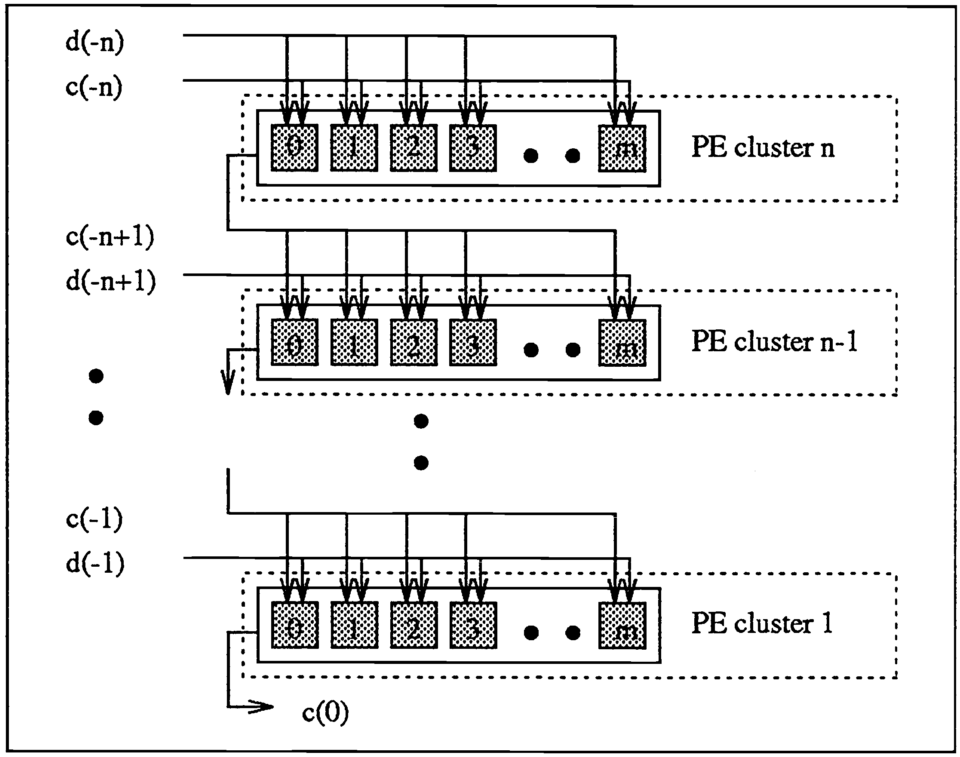
\includegraphics[width=0.8\textwidth]{fig/simd2.png}
    \caption{The pipeline of rows of PEs executing same instructions.
             The output of previous row serves as input for the next row
             of PEs to perform the next iteration of DWT.}
    \label{fig:simd2}
\end{figure}


From the perspective of parallel execution, this implementation uses
a pipeline pattern to achieve great parallelism.
%
As we discussed in class, the amount of parallelism achieved depends on
the number of iterations of DWT we could perform on the input signal.
%
This implementation might not be able to make use of all PEs if run on 
a very large system with many rows of PEs.


The experiment shows that the parallel implementation has a better 
performance than that of a serial implementation on the SPARC 1 workstation,
whose processor is at least 100 times faster than that of the MasPar.
%
Scalability wise, this pipeline implementation is able to keep good speedups
when the problem size grows.
%
This is because larger problems naturally enables more iterations of DWT
to apply on.
%
As a result, the execution pipeline has more steps, and can run more efficiently.

\label{sec:simd}

\section{Shared Memory Architecture}
When performing DWT, the calculation of each coefficients depends only 
on a few input elements from its neighbors (see stencil pattern 
discussion in Section~\ref{sec:bg}).
%
This property makes the calculation of DWT fit in the 
Shared Memory Architecture (SMA) very well, 
by assigning each PE a small chunk of the input signal array
to operate on.
%
Research works from Kutil et. al. and Lucka et. al. both employ
this parallel scheme~\cite{kutil1999hardware, lucka2000parallel}.

Experiments by Kutil et. al. on the SGI POWERChallengeGR machine showed 
a linear speedup up to 10 PEs, while the parallel efficiency drops 
dramatically with more PEs.
%
The researchers than decided that the efficiency was hurt by 
cache misses when more PEs were involved in.
%
These observations and analyses are confirmed by Lucka et. al.
%
Their experiments and analyses showed similar speedup patterns
and performance impact by cache misses.

\label{sec:sma}

\bibliographystyle{plainyr} 
%\bibliographystyle{plain}
\bibliography{main}
\end{document}

